
\hfill
\begin{figure}[htbp]
\begin{center}
%\resizebox{0.5\textwidth}{!}{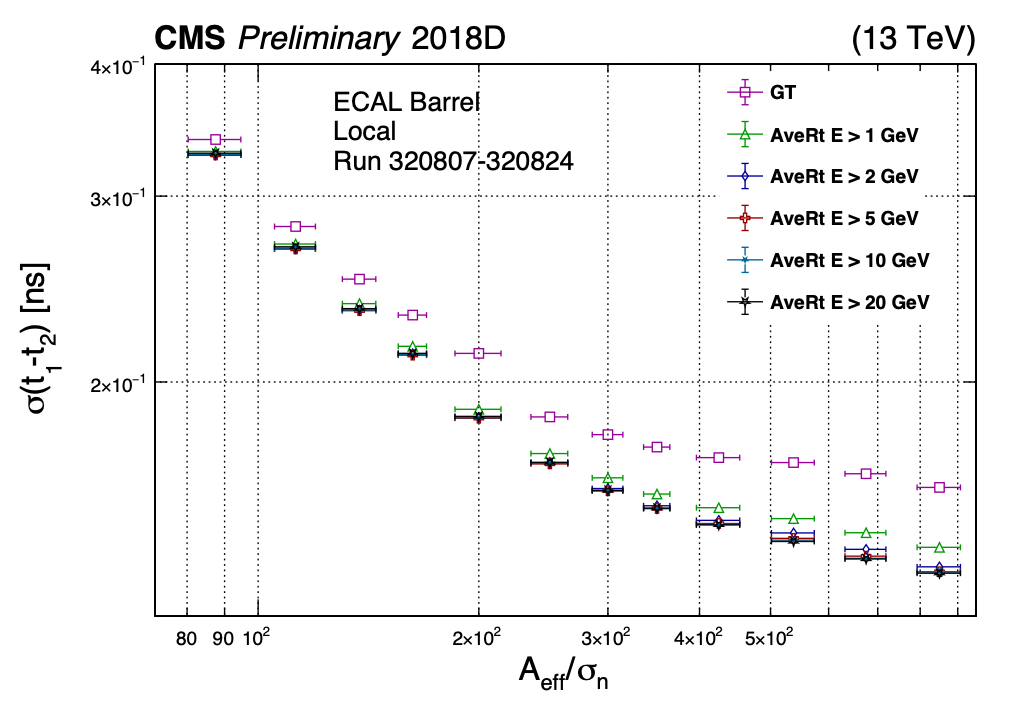
\includegraphics{fig/sec_method/e5cali.png}}
\resizebox{0.7\textwidth}{!}{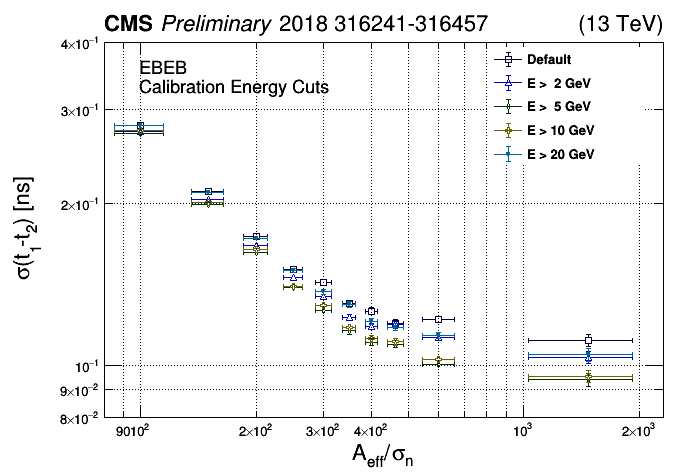
\includegraphics{fig/sec_method/tr_kucc_18s_ecut_v25_01122021174016.png}}
\caption{Same RO resolution with external calibration applied to default CMSSW timing reconstruction. The external calibration is calculated by taking the average rechit time by channel for rechits that have a minimum energy of 5 GeV over all events in the runs for which the calibration is used. }
%for runs 320807 - 320604 in 2018D era 
\label{e5cali}
\end{center}
\end{figure}

In order to compare various timing algorithms it is necessary to calibrate the rechit times produced by the different timing algorithms in the same manner. Since, during development in Run 2,  it is not possible to run the default timing calibration present in CMSSW on the CC algorithm, an external calibration based on the average rechit time by channel was implemented. Rechits selected for the channel by channel average rechit time are required to have a minimum energy to reduce the effects of noise. As shown in Figure~\ref{e5cali}, several different values for this energy cut were studied with the default CMSSW time reconstruction method in selected runs from the 2018D era. It was found that a minimum energy cut above 5 GeV produced a negligible improvement in the resolution when the corresponding calibration is applied to the rechit times and a minimum energy threshold of 5 GeV are used for the external calibration. This external calibration is always used for the CC method prior to the implementation of a CC based calibration in CMSSW during Run 3. An external calibration based on times reconstructed with the ratio method is also used as an additional external calibration to the ratio method times in all cases where the two timing methods are compared and an external calibration was requited for the CC method. 

%It is also required that only rechits in a collection produced with the CC algorithm that had corresponding rechits in the default rechit collection were used in any comparison of the two timing methods and in the creation of the calibration. 
%To account for uncertainty introduced in the determination of the resolution when using this calibration, the $\Delta(SeedTime)$ in the plot of $\Delta(SeedTime)$ as a function of $A_{eff}/\sigma_{N}$ has a Gaussian smear applied using the width of the distribution from which the average rechit time, by channel, is taken for the calibration.

